\chapter{Methods for Fusing LLMs and KGs for Enhanced Factuality}
\label{chap:methods}

% Comment: This chapter details your core methodological contributions, drawing heavily 
% from "Answer Candidate Type Selection...", "Large Language Models Meet KGs...", 
% and the methodological aspects of "ShortPathQA...

This chapter delves into specific methodologies developed to fuse the generative capabilities of Large Language Models (LLMs) with the structured factual knowledge encoded in Knowledge Graphs (KGs). As discussed in Chapter~\ref{chap:introduction}, while LLMs excel at text generation and comprehension, they often struggle with factual accuracy and are prone to generating plausible-sounding but incorrect information, a phenomenon often referred to as hallucination~\cite{lin-etal-2022-truthfulqa, DBLP:conf/emnlp/RobertsRS20}. Fusing LLMs with external KGs presents a compelling strategy to mitigate these limitations by grounding model outputs in verified factual structures~\cite{DBLP:journals/tkde/PanLWCWW24}. This integration process, broadly termed LLM-KG fusion, aims to leverage the strengths of both paradigms: the fluency and contextual understanding of LLMs (parametric knowledge) and the precision and reliability of KGs (non-parametric knowledge)~\cite{DBLP:conf/acl/MallenAZDKH23}.

Several approaches exist for this fusion. Some methods focus on encoding graph structure directly, using techniques like Graph Convolutional Networks (GCNs) for tasks like graph-to-text generation. However, recent work suggests that LLMs themselves, with appropriate prompting or fine-tuning, can often outperform specialized GCN architectures, particularly in handling the nuances of language and reducing factual errors~\cite{iarosh-etal-2025-reducing, DBLP:conf/ijcai/0001LW0S0Y24}. Another direction involves injecting knowledge more directly into the LLM parameters using techniques like adapters, attempting to distill relational facts into the model itself~\cite{DBLP:journals/corr/abs-2002-01808}. A prominent and flexible approach involves using the KG as an external knowledge source during inference, often retrieving relevant subgraphs or paths and incorporating this information into the LLM's prompt or generation process~\cite{DBLP:conf/emnlp/KnowledgeAugmented}.

This chapter focuses specifically on methods developed throughout our research that fall primarily within this latter category of leveraging external KG information to guide LLM generation for factoid QA. We introduce two distinct techniques: first, Answer Candidate Type (ACT) Selection~\cite{DBLP:journals/corr/abs-2310-07008}, which uses the LLM's understanding of semantic types combined with KG constraints; and second, a method utilizing explicit KG path information~\cite{DBLP:journals/corr/abs-2310-02166}, {\color{red}TODO: Add ShortPathQA, and Jouranl PAPER HERE} which provides direct factual evidence to the LLM. These methods form the foundation for the work detailed in the subsequent sections, aiming to create more controllable and factually reliable QA systems.


\section{Answer Candidate Type Selection - find the correct answer by extracting the type of the answer from LLM generated candidates}
\label{sec:methods_type_selection}

While Large Language Models (LLMs) demonstrate impressive capabilities in various natural language tasks, their application to factoid Question Answering (QA) in a closed-book setting is often marred by factual inaccuracies and hallucinations \cite{DBLP:conf/emnlp/RobertsRS20, lin-etal-2022-truthfulqa}. Interestingly, however, even when an LLM fails to produce the correct factual answer, it often exhibits an understanding of the question's underlying intent and the semantic \textbf{type} of the expected answer. For instance, when asked "What is the official language of Brazil?", an LLM might incorrectly respond "Spanish" but correctly identify that the answer should be a \textbf{language}. Similarly, for "Who directed the movie Inception?", it might hallucinate a director's name but still understand the answer should be a \textbf{person} (specifically, a film director).

This observation suggests a potential avenue for improving factuality. If we can reliably predict the expected answer type, this information can serve as a valuable constraint. Knowing the type is particularly useful when combined with the main entity mentioned in the question. The correct answer entity within a Knowledge Graph (KG) is often located semantically "close" to the question entity, connected via specific relations, and, crucially, belongs to the expected semantic type. For example, knowing the question entity is "Brazil" and the answer type is `dbo:Language` significantly narrows down the plausible candidates within the KG compared to an unconstrained search or generation process.

This section presents our proposed approach, Answer Candidate Type~(ACT) Selection. We propose a universal approach to selecting the correct answer in the KGQA task by using any pre-trained large language model to generate answer candidates and to infer the type of expected answer. The answer candidate type selection pipeline shown in Figures~\ref{fig:act_selection:pipeline} and \ref{fig:act_selection:pipeline_example}.

\begin{figure}[h]
    \centering
    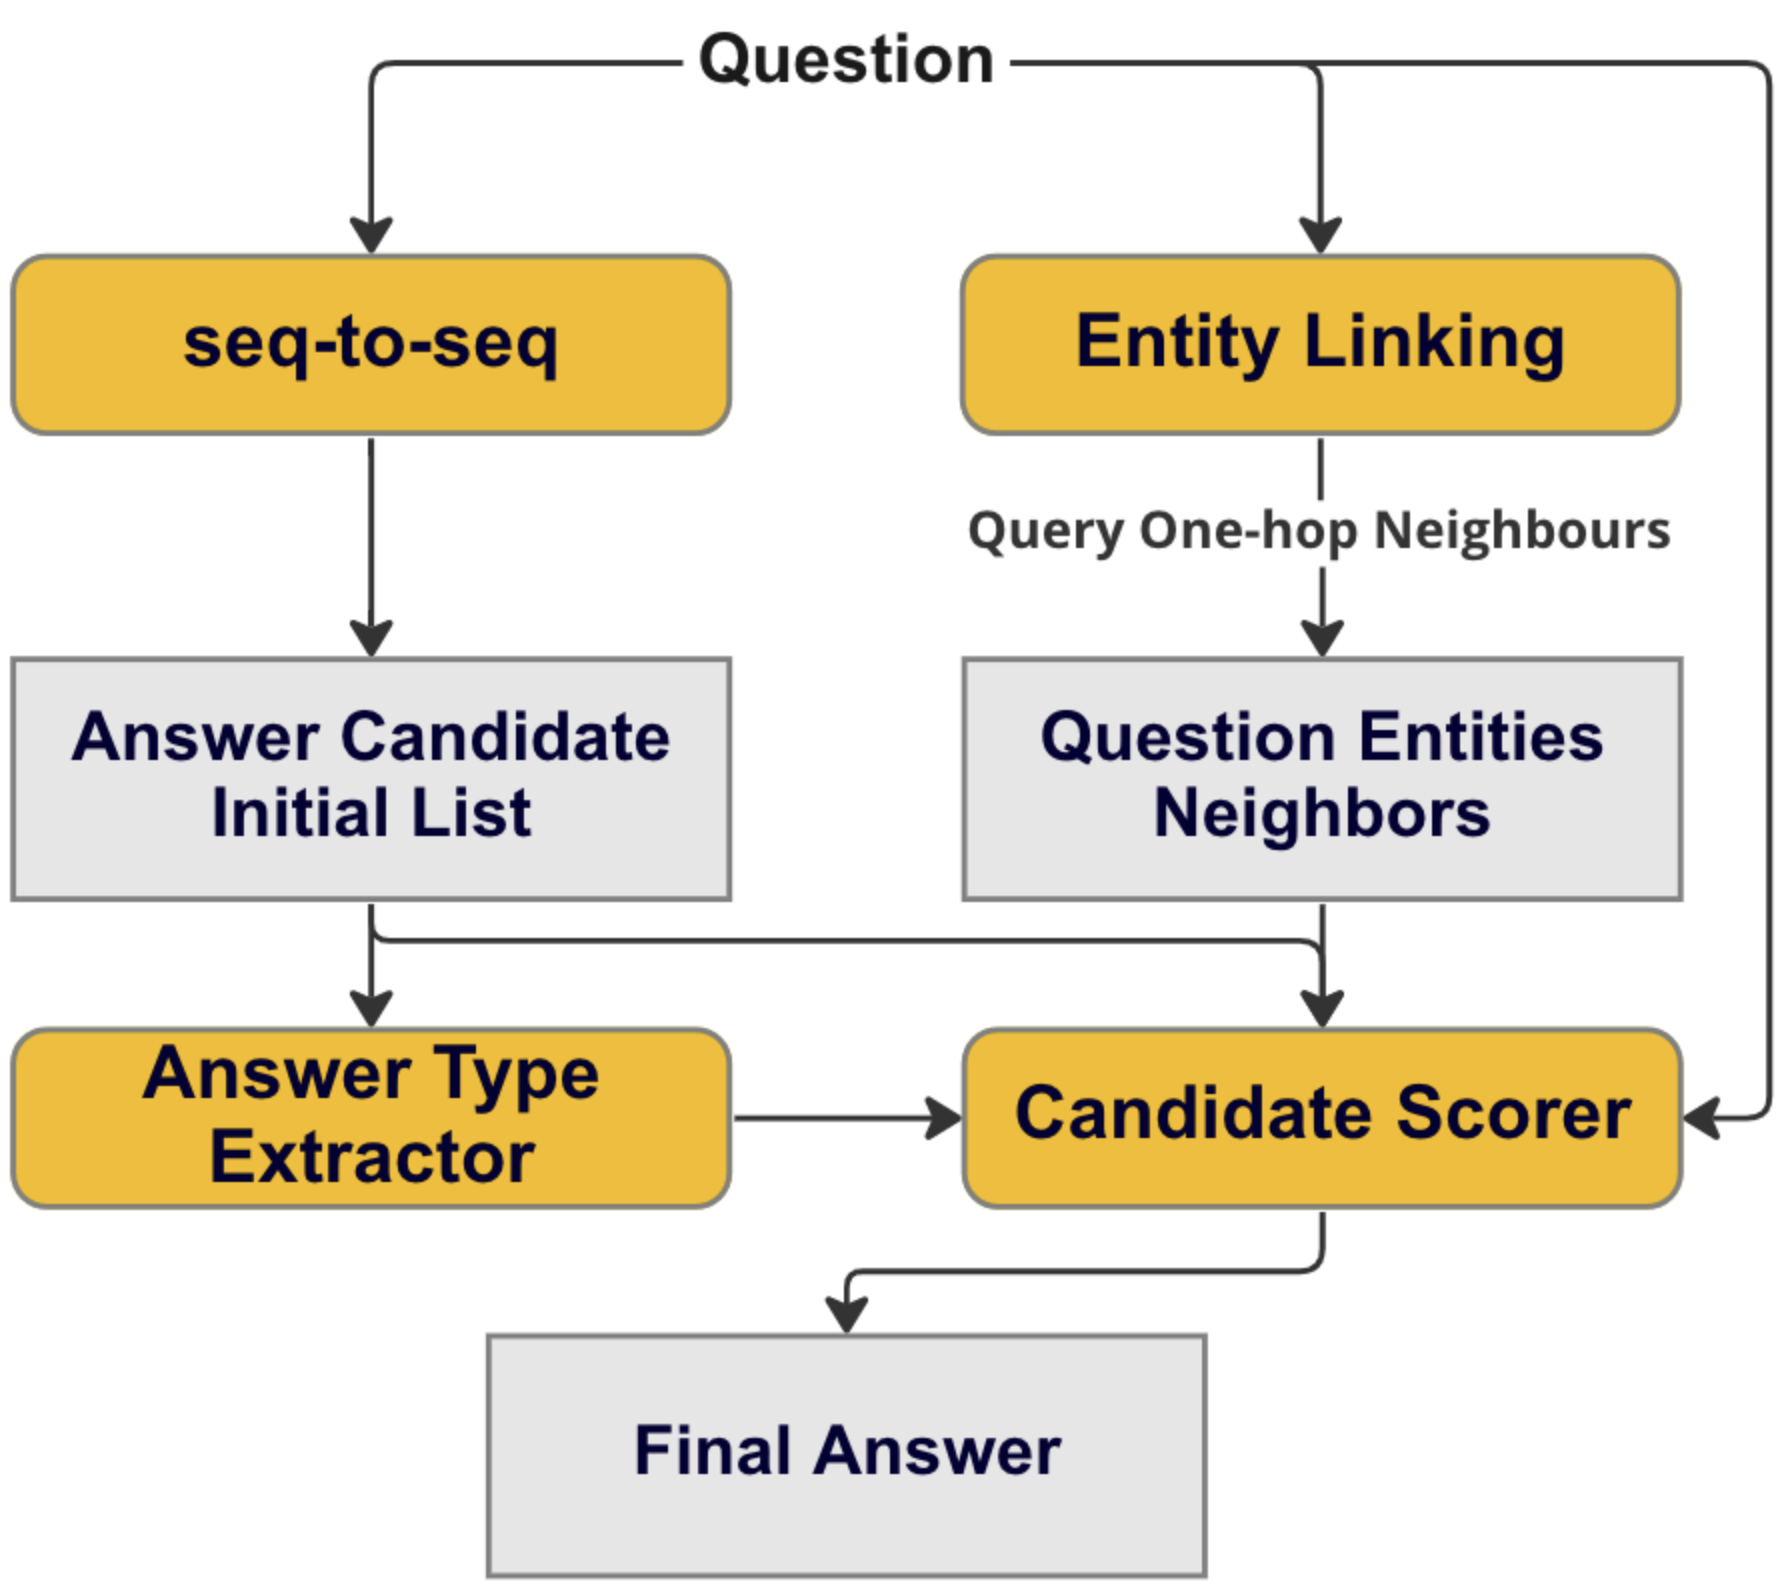
\includegraphics[width=0.85\textwidth]{act_selection/pipeline.png}
    \caption{ACT Selection Pipeline: (1) Put question to sequence to sequence language model to generate answer candidates, (2) Extract type from candidates, (3) Extract entities from the questions and query one-hop neighbors of the entities in the KG, (4) Filter candidates by type, (5) Select the best candidate.}
    \label{fig:act_selection:pipeline}
\end{figure}

\begin{figure}[h]
    \centering
    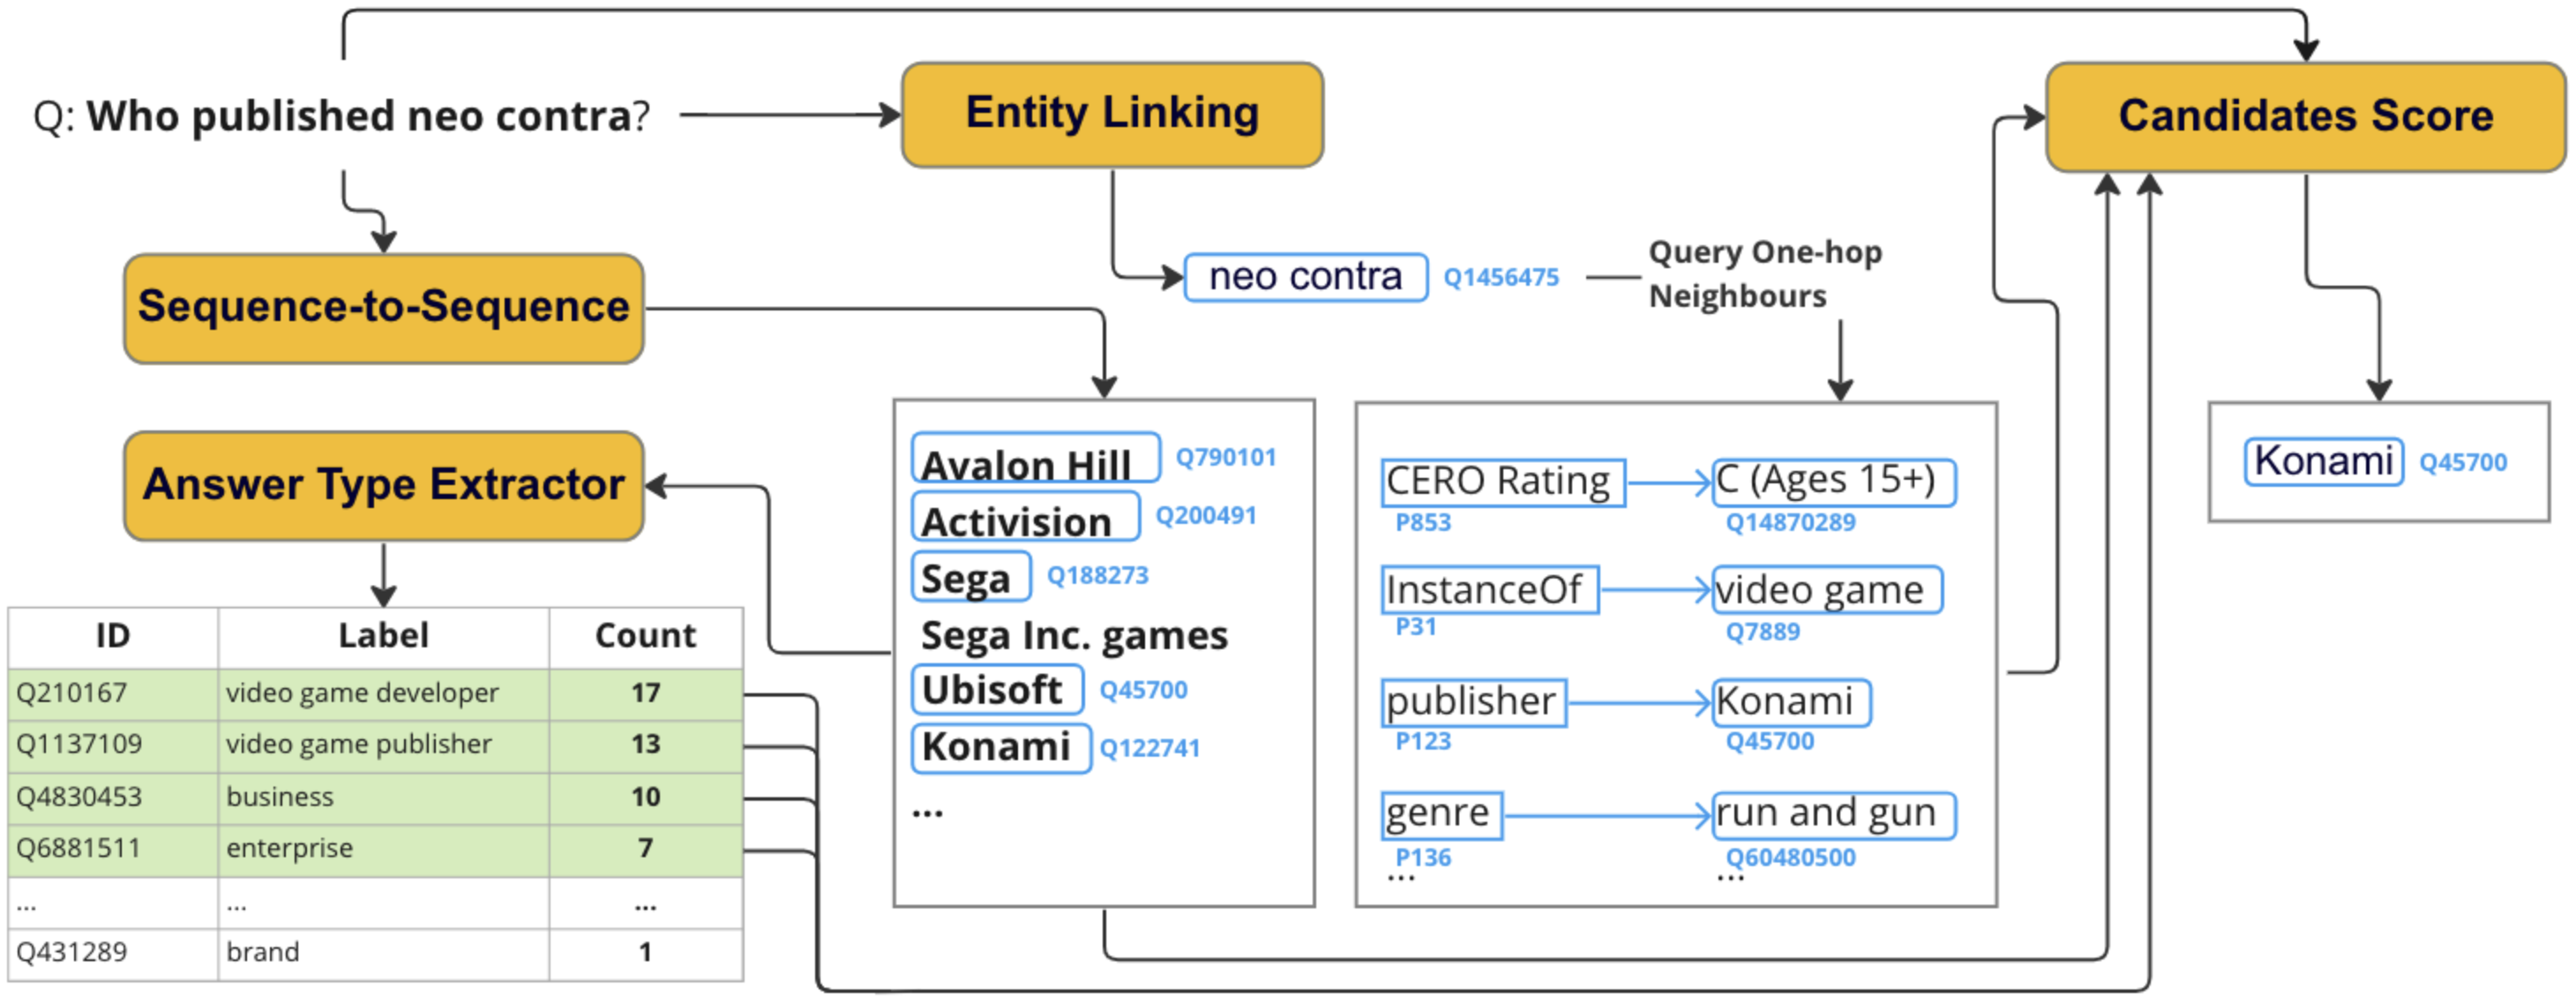
\includegraphics[width=0.95\textwidth]{act_selection/pipeline_example.png}
    \caption{The Answer Candidate Type (ACT) Selection pipeline for Knowledge Graph Question Answering (KGQA). The process combines a sequence-to-sequence model with knowledge graph-based entity linking and scoring to identify the correct answer, "Konami," as the publisher of "Neo Contra."}
    \label{fig:act_selection:pipeline_example}
\end{figure}

\subsection{Initial Answer Candidate List Generation} 
To increase the diversity of the generated results, we use Diverse Beam Search~\cite{DBLP:journals/corr/VijayakumarCSSL16-diverse-beam-search} to generate an initial list of answer candidates $C$. It often leads to a better exploration of the search space by ensuring that alternative answers are considered. It will discussed in more detail in Section~\ref{sec:methods_kg_path_fusion:expansion_of_generated_candidates}. We define the types of entities using the Wikidata property \texttt{instance\_of}~(P31). Note that an entity can be of multiple types. Finally, the initial list of answer candidates is used in the Answer Candidate Typing and the Candidate Scorer with the mined candidates. 

\subsection{Answer Candidate Typing} \label{act}
We rank all types by their frequency in the initial list of answer candidates. 
After that, we merge the top-$K$ most frequent types and similar types to the final list $T$.
Types similarity is calculated as cosine similarity between Sentence-BERT~\cite{reimers-2019-sentence-bert} embeddings of respective labels. The final types are defined as the ones where similarity is greater than a threshold.

A similar aggregation method using hypernyms (also known as ''is-a''  or ''instance-of'' relations) was used in the past to label clusters of words senses in distributional models~\cite{biemann2013text}: distributionally similar words share common hypernym and top common hypernyms are surprisingly good labels for sense clusters. The analogy in our method is that language models appear to produce a list of distributionally similar candidates.

\subsection{Entity Linking}
To enrich the list of candidates, we add all one-hop neighbors of the entities found in the question. For that, we use the fine-tuned spaCy Named Entity Recognition~(NER)\footnote{\url{https://spacy.io}.}

Based on a comprehensive review of state-of-the-art Named Entity Recognition (NER) systems \cite{vajjala-balasubramaniam-2022-really}, we evaluated the top three approaches: spaCy\footnote{\url{https://spacy.io}}, Stanza\footnote{\url{https://stanfordnlp.github.io/stanza/}}, and SparkNLP\footnote{\url{https://nlp.johnsnowlabs.com}}. Our analysis revealed that pre-trained NER models performed poorly on the Simple Question Wikidata (SQWD)~\cite{SQ_WD} dataset, with entity detection failure rates ranging from 64\% to 88\%. Among these systems, spaCy demonstrated the best performance, leading us to select its standard configuration\footnote{\url{https://spacy.io/usage/training/}} for further fine-tuning. The implementation of this pipeline required two critical pre-processing steps. First, we needed to identify the entity span to feed into the algorithm. This necessitated first extracting entity labels and their corresponding redirects, then locating these labels within the question text to determine spans. For entities without exact matches in the question, we employed fuzzy search techniques\footnote{\url{https://pypi.org/project/fuzzywuzzy/}}. Second, spaCy's training process requires entity type tags (e.g., PERSON for "Elon Musk", ORG for "Tesla" - following the BIO tagging scheme), which were not provided in the original datasets. We initially assigned the PERSON tag universally across all entities. Subsequent experiments with more precise entity type tagging did not yield significant improvements.
After extensive evaluation, we ultimately selected mGENRE \cite{decao2021multilingual} as our entity linking solution, which demonstrated superior performance compared to the NER-based approaches. mGENRE functions as an end-to-end entity linking system that eliminates the need for separate entity detection and disambiguation steps. Its multilingual autoregressive entity linking capabilities provided better accuracy and robustness across diverse question formulations in our experiments, making it a practical choice for our knowledge graph question answering pipeline.

\subsection{Candidates Scorer}
Finally, we calculate four scores for each entity from the answer candidate and rank them based on the weighted sum of the scores.
The scores are as follows:
% \begin{itemize}
    % \item
    \textbf{(1)~Type score} represents the size of the intersection between the set of types extracted from the answer candidates and the selected answer types. It is weighted by the number of selected answer types: $$S_\textrm{type}~=~\frac{|\textrm{Candidates' Types} \cap T|}{|T|}.$$

    % \item
\textbf{(2)~Forward one-hop neighbors score} $S_\textrm{neighbour}$ is  assigned 1 if the candidate is among the neighbors of the question entities, and 0 otherwise.

    % \item
\textbf{(3)~Text-to-Text answer candidate score} is determined by the rank of the candidate in the initial list $C$ generated by the Text-to-Text model divided by the size of the list: $$S_\textrm{t2t}~=~\frac{C.\textsc{}{index}(\textrm{Candidate})}{|C|}.$$

    % \item
\textbf{(4)~Question-Property Similarity score} $S_\textrm{property}$ measures the cosine similarity between the embeddings of the relevant property and the entire question. We employ Sentence-BERT~\cite{reimers-2019-sentence-bert} to encode the question, following a similar approach used for the Answer Candidate Type module.
% \end{itemize}
The four scores are calculated for each entity and then are combined to generate a final score that determines the entity's ranking. The answer with the highest weighted sum of scores in the candidate list is selected as the final answer:
%
$$S_\textrm{final} = S_\textrm{type} + S_\textrm{neighbour} + S_\textrm{t2t} + S_\textrm{property}.$$

% The weights for this sum can be estimated using logistic regression on a sample dataset in a future works.

% Text-to-Text models, despite occasionally providing incorrect answers, still yield answers of the correct type that can be utilized within the KGQA pipeline. This is demonstrated in the example depicted in Figure~\ref{fig:pipeline_example}.

% TODO: Добавить больше текста - заключение для метода 

% 3.2 Controllable Fusion using Knowledge Graph Paths
\section{Controllable Fusion using Knowledge Graph Paths}
\label{sec:methods_kg_path_fusion}

While constraining the answer type, as discussed in Section~\ref{sec:methods_type_selection}, provides a valuable signal for improving factuality, another powerful approach involves leveraging the explicit relational structure within the Knowledge Graph more directly. This section introduces methods based on the core idea of using KG subgraphs - a small part of the KG that contains the entities from the question, answer candidate generated by the LLM, and the shortest paths between them, drawing upon the work presented in \cite{DBLP:journals/corr/abs-2310-02166} and subsequent refinements focused on reranking 
{\color{red} TODO: add cite SWJ Reranking Answers of Large Language Models with Knowledge Graphs}.

The central motivation is to move beyond implicit knowledge within the LLM and provide explicit, verifiable evidence trails from the KG. Instead of solely relying on the LLM to generate a factually correct answer, we can use paths connecting entities mentioned in the question to potential answer entities within the KG as a strong indicator of factual consistency. This approach offers greater controllability and interpretability, as the KG path itself serves as evidence supporting a given answer.

The general pipeline for this fusion strategy, illustrated in Figure~\ref{fig:methods_kg_path_fusion:big_pipe}, involves several stages. First, relevant entities are identified within the input question. Second, candidate answers might be generated by an LLM, or potential answer entities are retrieved from the KG, focusing on entities connected to the question entities via relatively short paths. Crucially, features are extracted from these connecting paths (or the surrounding subgraph). These features capture information about the path structure and relations involved. Finally, these subgraph based features are used by a scoring or reranking model to evaluate the correctness of each candidate answer, ultimately selecting the answer best supported by the explicit structure of the Knowledge Graph. This section will detail the specific mechanisms developed for implementing this subgraph based fusion method.

\begin{figure}[htb]
    \centering
    \includegraphics[width=\columnwidth]{kg_path_fusion/new_paper_big_pipeline.pdf}
    \caption{The proposed method for reranking language model answers with KGs. The method includes subgraph extraction, features extraction, and various ranker approaches.}
    \label{fig:methods_kg_path_fusion:big_pipe}
\end{figure}
  
% In this section, we examine each component of the process in detail.
%  Firstly, we generate answer candidates using various LLMs and generate subgraphs, as discussed in Subsection~\ref{sec:subgraph_extract}. Next, in Subsection~\ref{sec:subgraph_features}, we will look at which attributes are used to rank responses.

\subsection{Answer Candidate Generation} \label{sec:methods_kg_path_fusion:expansion_of_generated_candidates}
As the subgraph extraction protocol requires answer candidates, we need a source of distinct answer candidates for each question, but most LLM approaches for QA, such as the one presented by \cite{DBLP:conf/coling/SenAS22-mintaka}, typically use \texttt{Greed Search} and evaluate the top-1 answer, it is important to note that the correct answer may not always be the top candidate. For example, the fine-tuned T5-XL-SSM~\cite{DBLP:conf/emnlp/RobertsRS20} model achieved higher Mean Reciprocal Rank (MRR) scores for our task, indicating that re-ranking could improve the top-1 results. 
However, even when using \texttt{Classical Beam Search}, the output is often minor variations of a single sequence, which may not generate enough unique answer candidates for the Question Answering task. Similar to the approach a little bit described in Section~\ref{sec:methods_type_selection}, we use Diverse Beam Search~\cite{DBLP:journals/corr/VijayakumarCSSL16-diverse-beam-search} to generate an initial list of answer candidates.

The formula~\ref{eq:methods_kg_path_fusion:diverse_beam_search} involves splitting the set of beams at time $t$ into $g$ disjointed subsets $Y_{[t]}^g$, and then selecting the candidate with the highest diversity penalty, which is calculated as the sum of a diversity penalty function $\Theta(y_{b,[t]}^g)$ over all candidates in the subset. Additionally, a dissimilarity term is included, which is calculated as the sum of a dissimilarity function $\Delta(y_{b,[t]}^g, Y_{[t]}^h)$ over all previous subsets $Y_{[t]}^h$ up to time $g-1$. The dissimilarity term is weighted by a parameter $\lambda_g$. This formula is used to optimize the selection of answer candidates in a computationally efficient manner.

\begin{equation}
    \begin{aligned}
        Y_{[t]}^g = \quad & \underset{y_1^{g}, \dots, y_{B\prime}^g \in Y_t^g} {\text{argmax}} \quad \underbrace{\sum_{b \in [B\prime]} \Theta(y_{b, [t]}^g)}_{\text{diversity penalty}} \\ 
        & + \underbrace{\sum_{h=1}^{g-1} \lambda_g \Delta(y_{b,[t]}^g, Y_{[t]}^h)}_{\text{dissimilarity term}},
    \end{aligned} 
    \label{eq:methods_kg_path_fusion:diverse_beam_search}
\end{equation}

% We apply {Diverse Beam Search} to the following LLMs: {T5-large-ssm}, {T5-XL-ssm}, {Mistral}, and {Mixtral} with $200$ beams, $20$ beam groups, and a $0.1$ diversity penalty. We extend our previous research~\cite{DBLP:conf/paclic/SalnikovLRNBMP23-originalpaper} by fine-tuning the proposed T5-like models and comparing them to more recent state-of-the-art models like Mistral and Mixtral, which should make our research more applicable to real-world use cases. T5-large-SSM and T5-XL-SSM were reported to be state-of-the-art both in the original Mintaka paper and our previous work, serving as a good baseline for comparison in this study.

% To finetune the T5-like models, we first train them on English questions for $10000$ steps, following the protocols outlined in the original Mintaka paper~\cite{DBLP:conf/coling/SenAS22-mintaka}. For the more state-of-the-art Mistral and Mixtral, we finetune with LoRA and train on English questions by generating the answer candidates with ``\textit{Answer as briefly as possible without additional information. [Question]}''. However, for the T5-like models, despite adhering to these protocols, we could not achieve the reported Hits@1 accuracy in the original paper. Despite this challenge, the main focus of the study is on the reranking aspect of the pipeline. Therefore, this paper's primary contribution is improving our fine-tuned models.

\subsection{Subgraph Extraction} \label{sec:subgraph_extract}
The main backbone of our approach is the procedure of subgraph extraction. We rely on the information conveyed in the relationships between question-answer pairs to improve the reranking of LLM generations. To further investigate how this relationship can improve performance, we employ a subgraph extraction algorithm that generates a KG's subgraph containing entities relevant to each question-answer pair and the shortest paths between them that contain relevant properties/relationships. 
% We extract various features that can be used for reranking in addition to the subgraphs. This section presents the subgraph extraction algorithm, the features derived from the subgraphs, and our reranking approaches.

\begin{figure}[htb]
    \centering
    \includegraphics[width=\columnwidth]{kg_path_fusion/ssp_to_sub.pdf}
    \caption{The proposed method for reranking language model answers with KGs. The method includes subgraph extraction, features extraction, and various ranker approaches.}
    \label{fig:methods_kg_path_fusion:subgraph_construction_example}
\end{figure}

For each question-answer candidate pair, the desired subgraph $G$ is mathematically defined as an induced subgraph of the Knowledge Graph. Thus, given our shortest paths from $e_i~\rightarrow~A$, where $e_i$ - entity extracted from question and $A$ - Answer. We can use the following Listing~\ref{alg:methods_kg_path_fusion:sub_extract} to extract $G$. Let us define $H$ as the set of all distinct nodes within our shortest paths $P_i$. We want to preserve all edges between the nodes within $H$. For all question-answer pairs, our objective is to retain the relationship between our question entities $E$ and answer candidate entity $A_i$. The process is schematically depicted at Figure~\ref{fig:methods_kg_path_fusion:subgraph_construction_example}.

\begin{ListingEnv}[p]
    \centering % Center the listing if desired
    \caption{Subgraph Extraction Algorithm} 
    \label{alg:methods_kg_path_fusion:sub_extract} 
    \begin{lstlisting}[basicstyle=\fontsize{10pt}{12pt}\selectfont\ttfamily] % Smaller font for code Require: entities, candidate

paths = []
For entity in entities:
    shortest_paths = get_shortest_path(entity, candidate)
    paths.extend(shortest_paths)

H = set of unique nodes in paths

G = new Graph()
Add nodes from H to G

For unique_node in H:
    unique_node_neighbors = get_neighbors(unique_node)
    For neighbor_node in unique_node_neighbors:
        If neighbor_node in H:
            Add edge (unique_node, neighbor_node) to G

Return G
    \end{lstlisting}
\end{ListingEnv}


\subsection{Features based on Extracted Subgraphs} \label{sec:methods_kg_path_fusion:subgraph_features}
After extracting subgraphs for all answer candidates of our LMs, we use all possible useful features for reranking. Referring to our previous study, we mainly focused on a simple text representation of the extracted subgraphs to rank our answer candidates. Thus, in this study, we propose extracting as many useful features as possible and analyzing each feature's importance in this reranking problem. We have divided the features into the following main categories: graph, text, and Graph2Text sequence features. 

\subsubsection{Graph Features} \label{sec:methods_kg_path_fusion:graph_features}
With our extracted subgraphs and their corresponding answer candidate, we seek to use the relationship from the subgraphs to classify the correct answer candidate. As the first simple baseline, we utilize graph features consisting of simple numerical subgraph statistics. We hypothesize that subgraphs with the correct answer will be less ``complex'' than subgraphs with the incorrect answer candidate. Therefore, we would want the graph features to convey the complexity of the respective subgraph. With a clear objective in mind, we experiment with the following graph features:  

\begin{itemize}
    \item \textbf{Number of nodes and edges}: basic statistics of the nodes and edges of graph $G$.
    \item \textbf{Number of cycles}: a cycle of graph $G$ is a non-empty path that starts from a given node and ends at the same node. 
    \item \textbf{Number of bridges}: a bridge of graph $G$ is an edge, where its deletion increases the number of connection components. 
    \item \textbf{Average shortest path}: the average of each shortest path between the question entity and the answer entity. 
    \item \textbf{Density}: measurement of the density of a graph, where the number of edges in a dense graph is close to the maximal number of edges (each pair of nodes is connected by an edge). The density $d$ for the graph $G$ is formulated as $d = \frac{m}{n(n-1)}$, where $n$ is the number of nodes and $m$ is the number of edges in $G$.
   \item \textbf{Katz centrality}~\cite{katz1953new}: measurement of the importance (or ``centrality'' - how ``central'' a node is in the graph) of a specific node $i$ in a graph $G$. The Katz centrality for node $i$ of graph $G$ is formulated as $x_i = \alpha \sum_{j} A_{ij} x_j + \beta$, where $A$ is the adjacency matrix of graph $G$ with eigenvalues $\lambda$, $\beta$ is the parameter that controls the initial centrality, and $\alpha < \frac{1}{\lambda_{\max}}$. 
    \item \textbf{PageRank}~\cite{page1999pagerank}: a popular algorithm used by Google to rank web pages in the search query by counting the number and quality of links to a page to determine an estimate of its importance. In graph theory, the ``web pages'' and ``links'' are synonymous with nodes and edges. 
\end{itemize}

\noindent We hypothesize that these features may provide ranker models with insights into the complexity of the respective subgraphs.


\subsubsection{Text Features} \label{sec:methods_kg_path_fusion:text_features} The ablation study showcased the importance of including the question within the text representation of the subgraph. Therefore, besides the simple graph features, we want to emphasize each question/answer pair without using extracted subgraphs. Thus, the text features represent the concatenation between the question and answer, separated by a semicolon --- ``\texttt{;}''. To use this simple concatenation for all ranker approaches, we encode the string using the MPNet\footnote{\url{https://huggingface.co/sentence-transformers/all-mpnet-base-v2}} embedding model~\cite{DBLP:conf/nips/Song0QLL20}.


\subsubsection{Graph2Text Sequence Features} \label{sec:methods_kg_path_fusion:g2t_seq} 
Given the vast amount of data contained in Knowledge Graphs, it is essential to convert this information into natural language to facilitate understanding and accessibility. Converting a graph into text, known as KG-to-text or Graph2Text, has demonstrated notable success in various applications~\cite{DBLP:journals/corr/abs-2309-11206}. Therefore, when generating text from a Knowledge Graph, it is crucial to analyze the underlying graph structure carefully to ensure accurate translation.

Without an obvious way of incorporating the question within the subgraphs, relying purely on the subgraphs to rerank is ineffective~\cite{DBLP:conf/paclic/SalnikovLRNBMP23-originalpaper}. Therefore, we address this issue by further exploration of different KG-to-text methods. The main objective is experimenting with various techniques to represent the extracted subgraphs more explicitly. For this type of textual feature, we researched and developed three methods for representing subgraphs as a text, including \textbf{Graph2Text Deterministic,  Graph2Text T5, and  Graph2Text GAP}.

Firstly, we employ the \textbf{Graph2Text Deterministic} approach, the most straightforward text linearization approach. In simple terms, the subgraphs are unraveled by their matrix representation. Firstly, to linearize, we convert the subgraph into its binary adjacency matrix. Let us call it matrix $A$. 
Given $n$ nodes in the subgraph, the resulting matrix's dimension will be $n \times n$. The matrix's element $[i, j]$ represents the existence of an edge between a node with index $i$ and a node with index $j$. Then, we replace the edges in the matrix with the edge label and call it $A'$. 
Adjacency matrices are typically implemented with graphs with numeric weights. The weights were string representing the relationship between our nodes. Thus, we represented the existence of an edge with $1$, then replaced in the edge with the string relationship.
%Let us call this adjacency matrix with edge information . 
Lastly, we unravel $A'$ row by row to produce our final sequence and add the triple (node\_from, edge, node\_to) to our final sequence. Listing~\ref{alg:methods_kg_path_fusion:sub2seq} summarizes the aforementioned steps. 

\begin{ListingEnv}[p]
    \centering % Center the listing if desired
    \caption{Subgraphs to Sequence - Graph2Text Deterministic} 
    \label{alg:methods_kg_path_fusion:sub2seq} 
    \begin{lstlisting}[basicstyle=\fontsize{10pt}{12pt}\selectfont\ttfamily] % Smaller font for code

Require: Subgraph G
Ensure: Text representation of subgraph Seq

adj_matrix = get_adjacency_matrix(G)
Seq = ""
# Assuming adj_matrix is n x n, where n is number of nodes
# and indices correspond to node IDs
For i in range(number_of_nodes(G)): 
    For j in range(number_of_nodes(G)):
        # Assuming 0 indicates no edge, non-zero indicates an edge
        If adj_matrix[i][j] != 0: 
            # Assuming G allows lookup by index i, j
            node_i_label = get_node_label(G, i) 
            node_j_label = get_node_label(G, j)
            # Get edge info (label/type) between node i and j
            edge_info = get_edge_info(G, i, j) 
            # Append triple to sequence string, separated by e.g., semicolon
            Seq += node_i_label + " " + edge_info + " " + node_j_label + "; " 
Return Seq
    \end{lstlisting}
\end{ListingEnv}

For the remaining two text linearization approaches, \textbf{Graph2Text T5} and \textbf{Graph2Text GAP}, we employ more complex neural-based models trained on the WebNLG~2.0 dataset~\cite{DBLP:conf/acl/GardentSNP17}. This dataset consists of instances, where each includes a Knowledge Graph from DBpedia~\cite{DBLP:conf/semweb/AuerBKLCI07} and a target text comprising one or more sentences that describe the graph. The test set is divided into partitions of seen (DBpedia categories present in the training set) and unseen (DBpedia categories not present in the training set). The statistics of this hand-crafted and human-verified dataset are described in detail in Table~\ref{tab:methods_kg_path_fusion:webnlg_label}. 

\begin{table}
    \centering
    \caption{Statistics of the WebNLG 2.0 parallel knowledge graph-to-text dataset.}
    
    \begin{subtable}[t]{0.48\textwidth}
    \centering
    \begin{tabular}{lr}
        \toprule
        \textbf{Entities} & 2,730 \\
        \textbf{Relations} & 354 \\
        \textbf{Triples} & 81,927 \\
        \bottomrule
    \end{tabular}
    \caption{Knowledge Graph statistics. Total number of KG components, number of tokens in the narratives.}
    \label{tab:kg_stats}
    \end{subtable}
    \hfill
    \begin{subtable}[t]{0.48\textwidth}
    \centering
    \begin{tabular}{lr}
        \toprule
        \textbf{Total} & 623,902 \\
        \textbf{Unique} & 8,075 \\
        \textbf{Entity} & 60\% \\
        \bottomrule
    \end{tabular}
    \caption{Texts statistics. The percentage of text entities represents the portion of the text that includes entity labels.}
    \label{tab:methods_kg_path_fusion:webnlg_label}
    \end{subtable}
\end{table}

The idea behind the \textbf{Graph2Text T5} approach is to extract informative and useful features from KGs using pre-trained text-to-text LMs. With the impressive capabilities of pretrained LMs in the text-to-text generation task, we seek to replicate such results in the graph-to-text scope. Our idea is built upon the analogous algorithm discussed in~\cite{DBLP:journals/corr/abs-2007-08426}. The authors tackle the graph-to-text generation task in this work with two popular text-to-text pre-trained LMs, BART and T5. These models have an encoder-decoder architecture, which makes them well-suited for conditional text generation tasks. To adapt these models for the graph-to-text task, the authors continue pre-training BART and T5 using the following approaches:

\begin{enumerate}
    \item Language Model Adaptation (LMA): the models are trained on reference texts that describe graphs, following the BART and T5 pre-training strategies.
    \item Supervised Task Adaptation (STA): the models are trained on pairs of graphs and their corresponding texts collected from the same or a similar domain as the target task --- graph-to-text in this case. 
\end{enumerate}

Building on the STA approach via T5 and WebNLG~2.0, we obtain graph-to-text sequences by first converting the graph into a sequence of tokens through linearization. We use the string ``convert the [graph] to [text]:'' to acquire this linearised sequence. This output sequence is then fed into the input sequence for the T5 model tuned on WebNLG~2.0. 
% For tuning Graph2Text T5 approach, we use the following hyperparameters: \textit{learning rate}: $1e^{-3}$, \textit{batch size}: 4, \textit{gradient accumulation steps}: 32, and \textit{Adam optimizer}. 

The \textbf{Graph2Text GAP} approach is based on the current state-of-the-art graph-to-text task, GAP, built on BART~\cite{DBLP:conf/coling/ColasAW22-GAP}. 
The main idea of GAP is a fully graph-aware encoding combined with the coverage of pre-trained LMs. The GAP KG-to-text framework fuses graph-aware elements into existing pre-trained LMs, capturing the advantages brought forth by both model types. The architecture of this solution consists of two main components:

\begin{enumerate}
\item \textbf{Global Attention}: to capture the graph's global semantic information, the graph’s components are first encoded using an LM. This allows the model to leverage the lexical coverage of pre-trained LMs.
\item \textbf{Graph-aware Attention}: to attend to and update the representations of entities, relations, or both, a topological-aware graph attention mechanism was introduced, which includes entity and relation type encoding.
\end{enumerate}

Applying the work of GAP, we first linearize the input graph into a text string by creating a sequence of all triples in the KG, interleaved with tokens that separate each triple and the triple's components (head, relation, and tail). Then, we use a transformer encoder to obtain vector representations. The first module in each transformer layer acts as a Global Attention and captures the semantic relationships between all tokens. Moreover, we use a Graph-aware Attention module to capture the sparse nature of adjustment in a graph and apply it to entity and relation vectors from word vectors. By proposing this flexible framework, where graph-aware components can be interchanged, the current architecture aims to generate coherent and representative text descriptions of the KG. Like the Graph2Text T5 approach, we pretrain the model on the WebNLG~2.0 dataset and get the final predictions through the fine-tuned model. 
% For finetuning the Graph2text GAP approach, we use the following hyperparameters: \textit{learning rate}: $2e^{-5}$, \textit{batch size}: 16; \textit{beam size}: 5, \textit{Adam Optimizer}, 50 \textit{nodes}, and 60 \textit{relations}.


% In this research, we introduce the more complex neural-based graph-to-text approach to explore further the reranking capabilities of the textual representation of our extracted subgraphs. The initial rudimentary text linearization approach has already achieved state-of-the-art Hits@1. We look for a more complete case study on reranking the text linearization with these two neural-based linearization approaches. To further digest the two methods, a comparison between the Graph2Text T5 and Graph2Text GAP sequences can be seen in the table ~\ref{tab:example_of_predictions_label}. Additionally, for better visualization, we implement a web application that automatically applies the T5 and GAP approaches to the desired subgraph, discussed in detail in Section ~\ref{sec:webapp}.
 

% \input{tabs/graph2text_examples}
% All three variation of Graph2Text Sequence features are further encoded with MPNet embedding model~\cite{DBLP:conf/nips/Song0QLL20}, discussed more in \ref{appx:detailed_results}. Moreover, motivated by our previous research, we employ context and highlight these Graph2Text sequences, discussed further in \ref{hl_context}.


% 3.3 Experimental Design and Baselines
\section{Experimental Design and Baselines}
\label{sec:methods_experimental_design}
% Comment: Describe the experimental setup used to evaluate the methods in 3.1 and 3.2. 
% Specify the datasets used (you might briefly introduce the motivation for ShortPathQA 
% here, leading into the next chapter), the evaluation metrics focused on factuality 
% and accuracy, and the baseline models (including perhaps zero-shot/few-shot LLMs, 
% and simpler KGQA systems).


% 3.4 Results and Analysis: Demonstrating Factuality Improvements
\section{Results and Analysis: Demonstrating Factuality Improvements}
\label{sec:methods_results}
% Comment: Present the quantitative results comparing your methods against baselines. 
% Crucially, analyze *why* your methods work, using examples and error analysis to 
% show how KG fusion mitigates specific failure modes of standalone LLMs (e.g., 
% hallucinations, factual errors). Discuss the trade-offs of each method. 